\newpage
\section{{\textcolor[RGB]{255,0,0}{This is RGB red text.}}}

For $x \in[r_{i-1},r_{i}]$ \\
$r(x)={\tilde{a}}_{1}x+{\tilde{b}}_{1}+\sum_{j=2}^{m}{\tilde{a}}_{j}(x-{\tilde{b}}_{j})_{+}$

\hrulefill

$\begin{array}{l}{{\mathsf{For}\;x\in[r_{i-1},r_{i}]}}\\ {{r(x)={\tilde{a}}_{1}x+{\tilde{b}}_{1}+\sum_{j=2}^{m}{\tilde{a}}_{j}(x-{\tilde{b}}_{j})_{+}}}\end{array}$\\
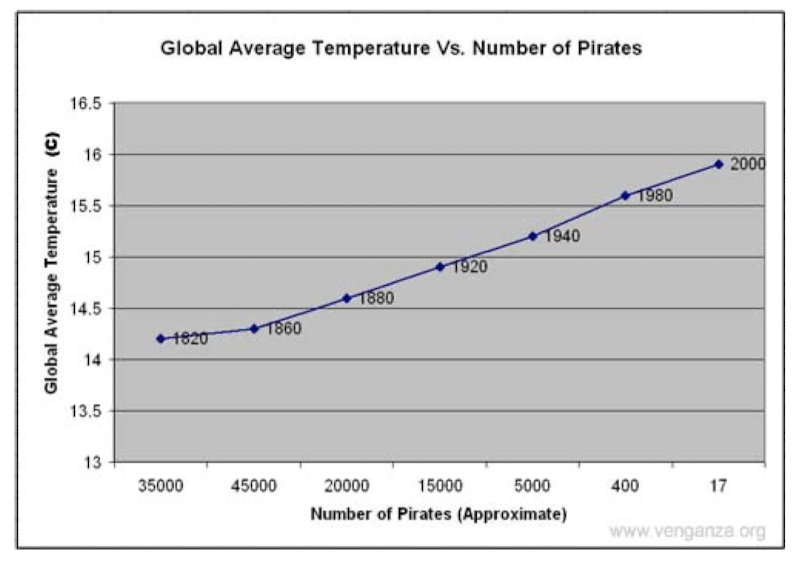
\includegraphics[width=\linewidth]{test_image}

\lipsum[1]

\noindent\dotfill

\lipsum[1]